%!TEX program = xelatex
\documentclass[tikz, border=3pt]{standalone}  % 核心配置:独立画布+智能裁剪
\usepackage{pgfplots}
\usepgfplotslibrary{colormaps}
\pgfplotsset{compat=1.18}

\begin{document}
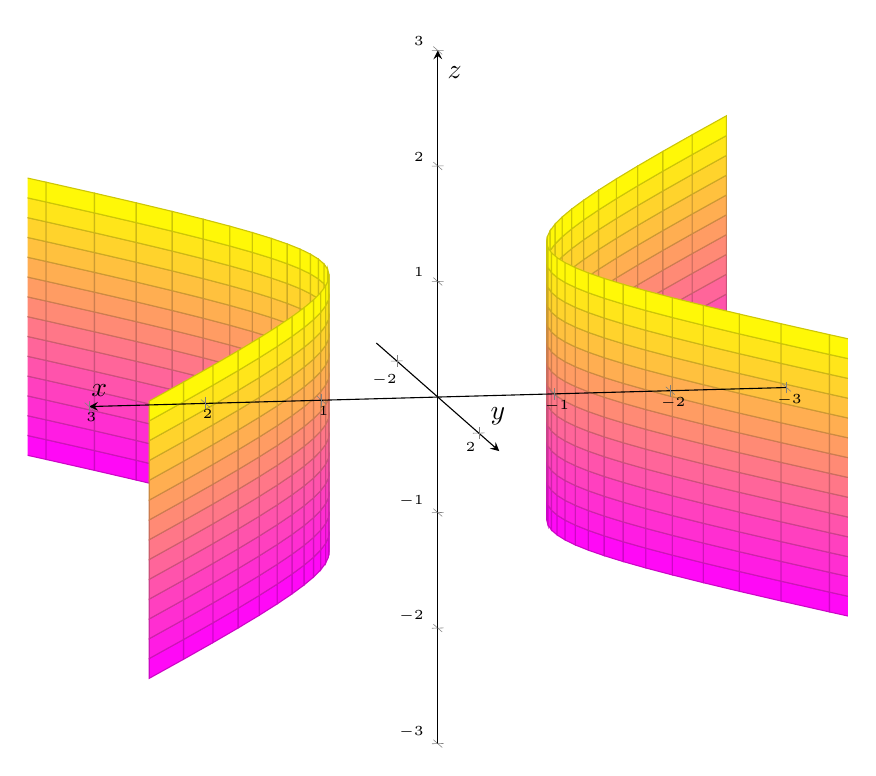
\begin{tikzpicture}
    \begin{axis}[
        colormap/spring,                     % 颜色映射声明移至axis环境
        view={170}{9},
        axis lines=center,
        axis on top,
        xlabel={$x$}, ylabel={$y$}, zlabel={$z$},
        xmin=-3, xmax=3, ymin=-3, ymax=3,    % 显式设置所有轴范围
        zmin=-3, zmax=3,
        width=12cm, height=12cm,
        tick label style={font=\tiny}
    ]
        % 右侧双曲面
        \addplot3 [ 
            surf, z buffer=sort,
            samples=30, samples y=15,        % 优化采样密度
            domain=-2:2, y domain=-1.2:1.2
        ] ({cosh(x)},{2*sinh(x)},{y});       % 简化系数写法
        
        % 左侧双曲面(对称部分)
        \addplot3 [
            surf, z buffer=sort,
            samples=30, samples y=15,
            domain=-2:2, y domain=-1.2:1.2
        ] ({-cosh(x)},{2*sinh(x)},{y});      % 负号实现对称
    \end{axis}
\end{tikzpicture}
\end{document}
